%%%%%%%% ICML 2019 EXAMPLE LATEX SUBMISSION FILE %%%%%%%%%%%%%%%%%

\documentclass{article}

% Recommended, but optional, packages for figures and better typesetting:
\usepackage{microtype}
\usepackage{graphicx}
\usepackage{subfigure}
\usepackage{booktabs} % for professional tables

% hyperref makes hyperlinks in the resulting PDF.
% If your build breaks (sometimes temporarily if a hyperlink spans a page)
% please comment out the following usepackage line and replace
% \usepackage{icml2019} with \usepackage[nohyperref]{icml2019} above.
\usepackage{hyperref}

% Attempt to make hyperref and algorithmic work together better:
\newcommand{\theHalgorithm}{\arabic{algorithm}}

% Use the following line for the initial blind version submitted for review:
\usepackage{icml2019}

% If accepted, instead use the following line for the camera-ready submission:
%\usepackage[accepted]{icml2019}

% The \icmltitle you define below is probably too long as a header.
% Therefore, a short form for the running title is supplied here:
\icmltitlerunning{Provable Overparameterized Neural Network Policy Gradient Method}

\usepackage{amssymb} %maths
\usepackage{amsmath} %maths
\usepackage{amsthm}
\usepackage{hyperref}
\usepackage[utf8]{inputenc} %useful to type directly diacritic characters
\usepackage[capitalize]{cleveref}
\crefname{prop}{Proposition}{Propositions}
\crefname{thm}{Theorem}{Theorems}
\crefname{lem}{Lemma}{Lemmas}
\crefname{algorithm}{Algorithm}{Algorithms}

\def\rva{{\mathbf{a}}}
\def\rvo{{\mathbf{o}}}
\def\rvr{{\mathbf{r}}}
\def\rvs{{\mathbf{s}}}
\def\rvu{{\mathbf{u}}}
\def\rvw{{\mathbf{w}}}
\def\rvx{{\mathbf{x}}}
\def\rvg{{\mathbf{g}}}
\def\rvo{{\mathbf{o}}}
\def\rvone{{\mathbf{1}}}
\def\rvzero{{\mathbf{0}}}
\def\rvtilder{{\tilde{\mathbf{r}}}}

\def\rvp{{\mathbf{p}}}

\def\pr{{\text{Pr}}}
\def\r{{\text{R}}}

\def\regret{{\text{Regret}}}

\newtheorem{thm}{Theorem}
\newtheorem{lem}{Lemma}
\newtheorem{defi}{Definition}
\newtheorem{prop}{Proposition}
\newtheorem{remk}{Remark}

\def\rvpi{{\boldsymbol{\pi}}}

\def\rmI{{\mathbf{I}}}
\def\rmW{{\mathbf{W}}}
\def\rmX{{\mathbf{X}}}

\def\sE{{\mathbb{E}}}
\def\sR{{\mathbb{R}}}
\def\sI{{\mathbb{I}}}

\def\gN{{\mathcal{N}}}
\def\gE{{\mathcal{E}}}
\def\gU{{\mathcal{U}}}

\DeclareMathOperator*{\argmax}{arg\,max}
\DeclareMathOperator*{\probability}{Pr}

\begin{document}

\twocolumn[
\icmltitle{Provable Overparameterized Neural Network Policy Gradient Method
}

% It is OKAY to include author information, even for blind
% submissions: the style file will automatically remove it for you
% unless you've provided the [accepted] option to the icml2019
% package.

% List of affiliations: The first argument should be a (short)
% identifier you will use later to specify author affiliations
% Academic affiliations should list Department, University, City, Region, Country
% Industry affiliations should list Company, City, Region, Country

% You can specify symbols, otherwise they are numbered in order.
% Ideally, you should not use this facility. Affiliations will be numbered
% in order of appearance and this is the preferred way.
\icmlsetsymbol{equal}{*}

\begin{icmlauthorlist}
\icmlauthor{Aeiau Zzzz}{equal,to}
\icmlauthor{Bauiu C.~Yyyy}{equal,to,goo}
\icmlauthor{Cieua Vvvvv}{goo}
\icmlauthor{Iaesut Saoeu}{ed}
\icmlauthor{Fiuea Rrrr}{to}
\icmlauthor{Tateu H.~Yasehe}{ed,to,goo}
\icmlauthor{Aaoeu Iasoh}{goo}
\icmlauthor{Buiui Eueu}{ed}
\icmlauthor{Aeuia Zzzz}{ed}
\icmlauthor{Bieea C.~Yyyy}{to,goo}
\icmlauthor{Teoau Xxxx}{ed}
\icmlauthor{Eee Pppp}{ed}
\end{icmlauthorlist}

\icmlaffiliation{to}{Department of Computation, University of Torontoland, Torontoland, Canada}
\icmlaffiliation{goo}{Googol ShallowMind, New London, Michigan, USA}
\icmlaffiliation{ed}{School of Computation, University of Edenborrow, Edenborrow, United Kingdom}

\icmlcorrespondingauthor{Cieua Vvvvv}{c.vvvvv@googol.com}
\icmlcorrespondingauthor{Eee Pppp}{ep@eden.co.uk}

% You may provide any keywords that you
% find helpful for describing your paper; these are used to populate
% the "keywords" metadata in the PDF but will not be shown in the document
\icmlkeywords{Machine Learning, ICML}

\vskip 0.3in
]

% this must go after the closing bracket ] following \twocolumn[ ...

% This command actually creates the footnote in the first column
% listing the affiliations and the copyright notice.
% The command takes one argument, which is text to display at the start of the footnote.
% The \icmlEqualContribution command is standard text for equal contribution.
% Remove it (just {}) if you do not need this facility.

%\printAffiliationsAndNotice{}  % leave blank if no need to mention equal contribution
\printAffiliationsAndNotice{\icmlEqualContribution} % otherwise use the standard text.

\begin{abstract}
In this paper, we propose a deep reinforcement learning algorithm which achieves nearly optimal finite time regret in the stochastic bandit setting. In our method, the agent maintains its action selection strategy in a parametric fashion. After enough exploration, a neural network is trained to minimized the empirical value related objectives using gradient updates. The policy is obtained from the exponential weight of learned logits. While our method is unlike standard bandit algorithms which directly utilize statistics from samples, we show that its finite time regret is nearly optimal up to log and constant factor. The results can be generalized to episodic MDPs and the state dependent bandit cases.
\end{abstract}

\section{Introduction}
\label{introduction}

Deep Reinforcement Learning (DRL) has recently achieved great successes, including games \citep{silver2016masteringA,silver2017masteringB,moravvcik2017deepstack,mnih2015human}, robotics \citep{lillicrap2015continuous,levine2016end}, just name a few. However, comparing with its brilliant achievements, the theoretical understanding of the mechanism behind DRL methods is not enough to explain its practical performance. 

DRL combines techniques in Deep Learning (DL) and Reinforcement Learning (RL) fields, to understand DRL, we need findings from both the DL and the RL sides.

On the RL side, it is well studied that under the bandit settings, and the tabular cases of the Markov decision process (MDP) setting, a number of algorithms enjoy favorable theoretical guarantees \citep{bubeck2012regret,sutton2018reinforcement}. In particular, either the optimal policies can be learned asymptotically, or within finite time, sublinear regret can be obtained. However, once it goes beyond the tabular cases, the theoretical results become much weaker. For example, Gradient Temporal Difference (GTD) with (non-)linear function approximations can only converge to the fixed points of projected Bellman operators \citep{sutton2009fast,sutton2009convergent,bhatnagar2009convergent}. While the performance of the fixed point policies can be arbitrarily bad without any further assumptions on the function approximations.

On the DL side, the empirical achievements are also much more advanced than the  theoretical results \citep{goodfellow2016deep}. However, there are still progresses in the expressiveness, optimization, and generalization aspects of DL theory. In particular, very recently, it has been discovered that, in supervised learning (regression and classification) settings, the training loss can be globally optimized (in linear convergence rate for $\ell_2$ loss in regression, and in constant time for classification) by gradient descent (GD) and stochastic gradient descent (SGD) method, given that the number of parameters in hidden layer is quite large, i.e., overparameterization. With some additional structured data distribution assumptions, the convergent training loss can be generalized to testing loss, making the neural network have provable generalization ability. 

To combine progresses in the DL and RL fields, we consider two main diferences between RL and supervised learning: (a) unlike the supervised learning settings, there are no true labels when learning RL agents; (b) to learn good agents, enough exploration is necessary.

In this paper, based on the recent progresses in overparameterized neural network optimization, we make one step forward to theoretically understanding DRL. In particular, we make the following contributions.
\begin{itemize}
    \item We prove that in bandit setting, with enough exploration, the widely-used policy gradient method, with policy net represented by a overparameterized two layer neural network (NN), achieves $O\left( \sqrt{T} \right)$ regret.
    \item We show that in episodic MDP setting, with the same exploration strategy and policy net as above, policy gradient method achieves $O\left( \sqrt{T} \right)$ regret.
    \item In many state dependent bandit and MDP settings, similar results also hold.
\end{itemize}

We would like to point that the above results can be generalized to policy net represented by multi-layered neural networks. Assuming a two layer NN policy is just for simplicity and conciseness. We provide the generalization to multi-layered NN in the appendix for completeness.

To our knowledge, our finding is the first convergence result for popular RL methods (here, policy gradient) with non-linear NN function approximations, which provides theoretical support for DRL methods. Our result is just beginning of understanding many other DRL methods (such as DQN \cite{mnih2015human}, A3C \citep{mnih2016asynchronous}, and PCL \citep{nachum2017bridging}), with more practical NN function approximations (e.g., less overparameterized), using many other policy optimization techniques (such as mirror descent, and relative entropy policy search).

The rest of the paper is organized as follows. Some proofs are deferred to appendix due to space limit.

\subsection{Notations}

Bold letters refer to vectors, and non-bold letters refer to scalars. For example, $u_{i,r} \in \sR$ is the $r$th component of vector $\rvu_i \in \sR^m$. $n$ is the total number of states, while $m$ is the total number of nodes in each hidden layer. $h$ is the total number of actions can be taken at each state. $\rvone$ means all-one vector, and $\rmI$ refers to identity matrix, with dimensions depends on the contexts.

Denote $[n] \triangleq \left\{ 1,2, \dots, n \right\}$. $\rvs_i \in \sR^d$, $i \in [n]$ refers to a state. $\rvw_r \in \sR^d$, $r \in [m]$ is a weight vector in the first hidden layer. $\rmW^\top \triangleq \left[ \rvw_1, \rvw_2, \dots, \rvw_m \right] \in \sR^{d \times m}$ is the weight matrix of the first hidden layer. $u_{i,r} \triangleq \rvw_r^\top \rvs_i$ is the $r$th node value of the first hidden layer. $\rva_k \in \sR^m$, $k \in [h]$ is a weight vector in the second hidden layer. In the paper, after the random initialization $\rva_k \sim \gU\left\{-1, +1\right\}$, $\rva_k$ will be fixed. This assumption is common in literature \citep{li2018learning,du2018gradientA,du2018gradientB,allen2018convergenceA,allen2018convergenceB}, and has been empirically verified that has no impact on the performance of trained neural networks \citep{hoffer2018fix}. Other initialization like $\rva_k \sim \gN(0, \rmI)$ also works. $\rmA^\top \triangleq \left[ \rva_1, \rva_2, \dots, \rva_h \right] \in \sR^{m \times h}$ is the weight matrix of the second hidden layer. $o_{i,k} \triangleq \sum\limits_{r=1}^{m}{a_{k,r} \cdot \sigma\left( u_{i,r} \right)}$ is the logit of the $k$th action for state $\rvs_i$, where $\sigma(\cdot) \triangleq \max\left\{ \cdot, 0 \right\}$ is the ReLU activation function. $\pi_{i,k} \triangleq f\left( o_{i,k} \right) \triangleq \frac{\exp\left\{ o_{i,k} \right\}}{\sum\limits_{k^\prime = 1}^{h}{\exp\left\{ o_{i,k^\prime} \right\}}}$ is the probability of choosing action $k$ at state $\rvs_i$, where $f(\cdot)$ is the softmax function. $\rvr_i \in \sR^h$ is the true reward vector at state $\rvs_i$. $\r_i^{\max} \triangleq \max\limits_{k \in [h]}\left\{ r_{i,k} \right\}$ is the maximum reward at state $\rvs_i$. $\rvtilder_i \triangleq \r_i^{\max} \cdot \rvone - \rvr_i$ is the true loss vector at state $\rvs_i$. Given stochastic policies $\rvpi \triangleq \left[ \rvpi_1, \rvpi_2, \dots, \rvpi_n \right] \in \sR^{h \times n}$, the expected loss is defined as,
\begin{equation}
\label{eq:expected_loss}
\begin{split}
    \ell \triangleq \frac{1}{n} \cdot \sum\limits_{i=1}^{n}{ \left( \r_i^{\max} - \rvpi_i^\top \rvr_i \right) } = \frac{1}{n} \cdot \sum\limits_{i=1}^{n}{ \rvpi_{i}^\top \rvtilder_{i} }.
\end{split}
\end{equation}

Without loss of generality, we assume $\rvr_i \in \left[ 0, 1 \right]^h$, $\forall i \in [n]$. Therefore $\rvtilder_i \in \left[ 0, 1 \right]^h$, $\forall i \in [n]$. For simplicity, we also assume $\rvr_i$ is a deterministic vector, $\forall i \in [n]$, while the results also generalize to random reward vectors. Finally, we use $\Delta_i \triangleq \max\limits_{k \in [h]}\left\{ \tilde{r}_{i,k} \middle| \tilde{r}_{i,k} > 0 \right\}$ to denote the reward gap between the optimal arm and the arm with the second largest reward at state $\rvs_i$, $\forall i \in [n]$.

\section{Main Results}

\subsection{Settings}

\subsubsection{Bandit}

We first analyze the standard bandit setting, i.e., $n = 1$ , and then generalize the results to many state dependent bandits setting. For simplicity, assume the reward $\rvr \in \sR^h$ is a deterministic vector. Using concentration the results can be generalized to random reward vectors, therefore recovering the stochastic bandit setting. Also we assume $r_k \in [0, 1]$, $\forall k \in [h]$.

In this setting, we use the NN policy to pull one arm $A_t \in [h]$ in each time step $t$, then observe the reward $r_{A_t}$. The policy net then uses the reward to update its weight vectors, using policy gradient method. After such $T$ steps, we are concerned with the regret,
\begin{equation*}
    \ell \triangleq \regret(\rvpi) \triangleq \r^{\max} \cdot T - \sum\limits_{t=0}^{T-1}{ \rvpi(t)^\top \rvr } = \sum\limits_{t=0}^{T-1}{ \rvpi(t)^\top \rvtilder }
\end{equation*}

\subsubsection{Episodic MDP}

In the Episodic MDP setting, in each time step, we use NN policy to take one action $A_t$, then observe a reward $R_{t+1}$ and next state $S_{t+1}$. After such $H$ steps, there is an ending state, and this trajectory terminates. Since we use policy gradient method (no value learning method here), the policy updates its weights using the cumulative reward collected from each trajectory. 


\subsection{Policy Gradient Method}

\begin{algorithm}[h]
   \caption{Policy Gradient Method Mixed with Uniform Exploration}
\label{alg:policy_gradient_uniform_exploration}
\begin{algorithmic}
   \STATE {\bfseries Input:} state feature vectors $\rvs_i$
   \STATE Initialize $\rvw_r \sim \gN\left( 0, \sigma \cdot \rmI \right)$, $\forall r \in [m]$, $\rva_k \sim \gN(0, \rmI)$, $\forall k \in [h]$.
   \FOR{$t=0$ {\bfseries to} $T-1$}
   \IF{$t < \sqrt{T}$}
   \STATE Uniformly randomly take action $A_{i,t}$. 
   \STATE Observe reward and next state.
   \ELSE
   \STATE Take action $A_{i,t} \sim \rvpi_{i}\left(\cdot \middle| S_{i,t} \right)$. 
   \ENDIF
   \STATE $\rvw_r(t+1) = \rvw_r(t) - \eta \cdot \frac{d\ell}{d \rvw_r(t)}$, $\forall r \in [m]$.
   \ENDFOR
\end{algorithmic}
\end{algorithm}

The objective of our analysis is the policy gradient method, mixed with uniform exploration, as shown in shown in \cref{alg:policy_gradient_uniform_exploration}. The reason why we need exploration will be explained later on, and technically it seems cannot be eliminated.

The policy gradient method works as follows. After initialization, the policy net $\rvpi$ will be updated using policy gradient calculated from collected reward. In the first $\sqrt{T}$ steps, actions are selected up to an uniform distribution over all actions. After that the NN policy $\rvpi$ is used to select actions.

\subsection{Main Results}
\label{subsec:main_results}

The first main result of the bandit setting is summarized in \cref{thm:main_result}.

\begin{thm}
\label{thm:main_result}
    Given a two layer NN policy $\rvpi$, with number of parameters $m \in \tilde{\Theta}\left( \frac{n^{10}}{c^4 \delta^4 \varepsilon^2} \right)$, $\eta \in \Theta\left( \frac{c^2 \delta^2}{16 n^4 h m \left( \log{\left(4m\right)} \right)^2} \right)$, the regret of \cref{alg:policy_gradient_uniform_exploration} satisfies $\sum\limits_{t=1}^{T}{ \rvpi_i\left( \rmW(t) \right)^\top \rvtilder_i } \le  \frac{8 n^4 \sqrt{h}}{c^2 \delta^2} \cdot \tilde{O}\left( \sqrt{T} \right)$.
\end{thm}
\begin{proof}
According to \cref{alg:policy_gradient_uniform_exploration}, the first $\sqrt{T}$ steps are played by uniformly taking actions, and they totally contribute $\sqrt{T}$ regret. After the first $\sqrt{T}$ steps, in expectation every arm is pulled $\frac{\sqrt{T}}{h}$ times, by \cref{thm:regret_convergence}, 
\begin{equation*}
\begin{split}
    \rvpi_i\left( \rmW(t) \right)^\top \rvtilder_i \le O\left( \frac{n^4}{\eta m c^2 \delta^2 \sqrt{T}} \right),
\end{split}
\end{equation*}
for $t = \sqrt{T}$. Denote $\varepsilon \triangleq \frac{n^4}{\eta m c^2 \delta^2 \sqrt{T}}$. By \cref{subsec:playing_phase}, $\rvpi_i\left( \rmW(t) \right)^\top \rvtilder_i \le \varepsilon$, $\forall t \ge \sqrt{T}$. Therefore the regret can be upper bounded by the sum of two parts,
\begin{equation*}
\begin{split}
    \sum\limits_{t=1}^{T}{ \rvpi_i\left( \rmW(t) \right)^\top \rvtilder_i } &\le \sqrt{T} \cdot 1 + \left(T - \sqrt{T} \right) \cdot \varepsilon \\
    &\le \frac{8 n^4 \sqrt{h}}{c^2 \delta^2} \cdot \log{\left(4m\right)} \cdot \sqrt{T} \\
    &\le \frac{8 n^4 \sqrt{h}}{c^2 \delta^2} \cdot \tilde{O}\left(\sqrt{T}\right). \qedhere
\end{split}
\end{equation*}
\end{proof}

\section{Theoretical Analysis}

We present more detailed analysis than \cref{subsec:main_results}. We first show the bandit case. Note that in the proof of \cref{thm:regret_convergence}, the $T$ steps are divided into two parts. In the first $\sqrt{T}$ exploration phase, we uniformly sample actions, and use collected rewards to make the expected regret of NN policy converge to smaller than $\varepsilon$. And in the second commit phase, we use NN policy to play, and because of the expected reward is small, we have the gradient norm lower bounded by positive constant times regret, so the NN policy will keep improving itself. Therefore our analysis will also be partitioned into two parts.

\subsection{Exploring Phase}
\label{subsec:exploring_phase}

In the exploring phase, we uniformly sample actions and rewards to update NN policy. The convergence of policy regret mainly relies on the following ``smoothness" like property over NN weights.

\begin{lem}
\label{lem:smoothness}
    Given weights $\rmW \triangleq \left[ \rvw_1, \rvw_2, \dots, \rvw_m \right]$, and $\rmW^\prime \triangleq \left[ \rvw_1^\prime, \rvw_2^\prime, \dots, \rvw_m^\prime \right]$. Denote $\rvpi_i\left( \rmW \right)$ and $\rvpi_i\left( \rmW^\prime \right)$ as the neural network policies parameterized by $\rmW$ and $\rmW^\prime$, respectively. $\forall i \in [n]$,
\begin{equation*}
\begin{split}
    &\rvpi_i\left( \rmW^\prime \right)^\top \rvtilder_i \le \rvpi_i\left( \rmW \right)^\top \rvtilder_i + \left\langle \frac{d \rvpi_i\left( \rmW \right)^\top \rvtilder_i }{d\left( \rmW \right)}, \rmW^\prime - \rmW \right\rangle \\
    &\qquad + 4 \sqrt{m \log{\left(4m\right)}} \cdot \rvpi_i\left( \rmW \right)^\top \rvtilder_i \cdot \left\| \rmW^\prime - \rmW \right\|_F \\
    &\qquad + 4 h m \log{\left(4m\right)} \cdot \left\| \rmW^\prime - \rmW \right\|_F^2.
\end{split}
\end{equation*}
\end{lem}

Combining this smoothness condition with other objective properties like convexity one can prove convergence results. However, the policy regret is non-convex function of weights. Therefore we need the recent results in overparameterized NN optimization, i.e., the gradient coupling and gradient (lower) bounds.

\begin{lem}
\label{lem:gradient_coupling}
	Define the pseudo gradient as,
\begin{equation*}
\begin{split}
	\frac{d \tilde{\ell}}{d \rvw_r(t)} &\triangleq \frac{1}{n} \cdot \sum\limits_{i=1}^{n}{ \sum\limits_{k=1}^{h}{ \tilde{r}_{i,k} \cdot \pi_{i,k}(t) \cdot \left( \sum\limits_{k^\prime = 1}^{h}{ a_{k^\prime,r}  \cdot v_{k^\prime,k,i}(t) } \right) } } \\
	&\qquad { { \cdot \sI\left\{ \rvw_r(0)^\top \rvs_i > 0 \right\} \cdot \rvs_i } },
\end{split}
\end{equation*}
where $v_{k^\prime,k,i}(t)$ is defined as,
\begin{equation*}
	v_{k^\prime,k,i}(t) = \begin{cases}
    1 - \pi_{i,k^\prime}(t), & \text{if $k^\prime = k$}, \\
    - \pi_{i,k^\prime}(t), & \text{otherwise}.
  \end{cases}
\end{equation*}
	For any $\tau > 0$, with probability at least $\frac{1}{2} \cdot \left( 1 - \frac{\sqrt{2}n\tau}{\sqrt{\pi}\sigma} \right)$, $\forall t \in O\left(\frac{\tau}{\eta  \sqrt{\log{m}}}\right)$, $\forall r \in [m]$,
\begin{equation}
	\frac{d\ell}{d \rvw_r(t)} = \frac{d \tilde{\ell}}{d \rvw_r(t)}.
\end{equation}
\end{lem}

The true gradient can be calculated as,
\begin{equation*}
\begin{split}
    \frac{d\ell}{d \rvw_r(t)} &= \frac{1}{n} \cdot \sum\limits_{i=1}^{n}{ \sum\limits_{k=1}^{h}{  \tilde{r}_{i,k} \cdot \pi_{i,k}(t) \cdot \left( \sum\limits_{k^\prime = 1}^{h}{ a_{k^\prime,r}  \cdot v_{k^\prime,k,i}(t) } \right) }} \\
    &\qquad  {{ \cdot \sI\left\{ \rvw_r(t)^\top \rvs_i > 0 \right\} \cdot \rvs_i } }.
\end{split}
\end{equation*}

\cref{lem:gradient_coupling} means $\sI\left\{ \rvw_r(t)^\top \rvs_i > 0 \right\} = \sI\left\{ \rvw_r(0)^\top \rvs_i > 0 \right\} $ for bounded time steps $t$ with constant probability, therefore the true gradient can be replaced with the simpler pseudo gradient.

The next lemma shows that the true gradient norm is upper bounded by regret, which is quite standard.

\begin{lem}
\label{lem:gradient_upper_bound}
With probability at least $\frac{1}{2}$,
\begin{equation*}
\begin{split}
	\left\| \frac{d\ell}{d \rvw_r(t)} \right\|_2 \le \frac{2 \sqrt{\log{\left(4m\right)}}}{n} \cdot \sum\limits_{i=1}^{n}{ \rvpi_{i}(t)^\top \rvtilder_i }.
\end{split}
\end{equation*}
\end{lem}

Now comes the key part of the recent progresses of overparameterized NN optimization theory, with constants probability, the pseudo gradient norm is lower bounded by the loss. However, due to the inherent difference of RL and supervised learning, our result contains an exploration item, which lead to the necessity of the exploration phase in \cref{alg:policy_gradient_uniform_exploration}. 

\begin{lem}
\label{lem:gradient_lower_bound}
	Denote $i^*(t) \triangleq \argmax\limits_{i \in [n]}\left\{\rvpi_i(t)^\top \rvtilder_i \right\}$, $k^*(t) \triangleq \argmax\limits_{k \in [h]}\left\{ r_{i^*(t),k} \right\} = \r_{i^*(t)}^{\max}$, i.e., the optimal arm of state $i^*(t)$. If $\pi_{i^*(t), k^*(t)}(t) > c > 0$, where $c$ is an exploration constant, then with probability $\Omega\left( \frac{\delta}{n} \right)$,
\begin{equation*}
\begin{split}
	\left\| \frac{d\tilde{\ell}}{d \rvw_r(t)} \right\|_2 \ge \Omega\left( \frac{c\delta}{n^2} \right) \cdot \rvpi_{i^*(t)}(t)^\top \rvtilder_{i^*(t)} .
\end{split}
\end{equation*}
\end{lem}

\cref{lem:gradient_lower_bound} is a generalization of recent overparameterized NN optimization results into the RL field. With this result, once the policy regret is large, with enough exploration of the optimal action (the constant $c$ here), the pseudo gradient norm will also be large (with constant probability). Therefore, combining \cref{lem:gradient_lower_bound} with \cref{lem:gradient_coupling}, we can get the true gradient norm is also large, which is necessary for objective progress and regret convergence. Using all the lemmas presented in this section, we get the convergence result for the exploring phase.

\begin{thm}
\label{thm:regret_convergence}
    Assume $m \in \tilde{\Theta}\left( \frac{n^{10}}{c^4 \delta^4 \varepsilon^2} \right)$, $\eta \in \Theta\left( \frac{c^2 \delta^2}{16 n^4 h m \left( \log{\left(4m\right)} \right)^2} \right)$, after $t \in O\left( \frac{n^4}{\eta m c^2 \delta^2 \varepsilon} \right)$ iterations, $\rvpi_i\left( \rmW(t) \right)^\top \rvtilder_i \le \varepsilon$.
\end{thm}
\begin{proof}
    By \cref{lem:gradient_coupling}, let $\tau = \frac{\sigma}{n}$, there is $\Omega\left( m \right)$ of $\rvw_r(t)$ such that $\left\| \frac{d\ell}{d \rvw_r(t)} \right\|_2 = \left\| \frac{d\tilde{\ell}}{d \rvw_r(t)} \right\|_2$, $\forall t \in O\left( \frac{\sigma}{\eta n \sqrt{\log{m}}} \right)$. Let $\rmW(t+1) = \rmW(t) - \eta \cdot \frac{d \ell}{d \rmW(t)}$, by \cref{lem:smoothness},
\begin{equation*}
\begin{split}
    &\rvpi_i\left( \rmW(t+1) \right)^\top \rvtilder_i \le \rvpi_i\left( \rmW(t) \right)^\top \rvtilder_i - \eta \cdot \left\| \frac{d \ell}{d \rmW(t)} \right\|_F^2 \\
    &\qquad + 4 \sqrt{m \log{\left(4m\right)}} \cdot \rvpi_i\left( \rmW \right)^\top \rvtilder_i \cdot \eta \cdot \left\| \frac{d \ell}{d \rmW(t)} \right\|_F \\
    &\qquad + 4 h m \log{\left(4m\right)} \cdot \eta^2 \left\| \frac{d \ell}{d \rmW(t)} \right\|_F^2 \\
    &\le \rvpi_i\left( \rmW(t) \right)^\top \rvtilder_i - \eta \cdot \sum\limits_{r=1}^{m}{ \left\| \frac{d\ell}{d \rvw_r(t)} \right\|_2^2 } \\
    &\qquad + 4 \sqrt{m \log{\left(4m\right)}} \cdot \rvpi_i\left( \rmW \right)^\top \rvtilder_i \cdot \eta \cdot \sum\limits_{r=1}^{m}{ \left\| \frac{d\ell}{d \rvw_r(t)} \right\|_2 } \\
    &\qquad + 4 h m \log{\left(4m\right)} \cdot \eta^2 \cdot \sum\limits_{r=1}^{m}{ \left\| \frac{d\ell}{d \rvw_r(t)} \right\|_2^2 } \\
    &\le \rvpi_i\left( \rmW(t) \right)^\top \rvtilder_i - \left( \rvpi_i\left( \rmW(t) \right)^\top \rvtilder_i \right)^2 \\
    &\cdot \left[ \frac{\eta m c^2 \delta^2}{n^4} - 8 \eta m \sqrt{m} \log{\left(4m\right)} - 16 \eta^2 h m^2 \left( \log{\left(4m\right)} \right)^2 \right] \\
    &= \rvpi_i\left( \rmW(t) \right)^\top \rvtilder_i - \left( \rvpi_i\left( \rmW(t) \right)^\top \rvtilder_i \right)^2 \cdot \Omega\left( \frac{\eta m c^2 \delta^2}{n^4} \right).
\end{split}
\end{equation*}
Divide $\left( \rvpi_i\left( \rmW(t+1) \right)^\top \rvtilder_i\right) \cdot \left( \rvpi_i\left( \rmW(t) \right)^\top \rvtilder_i \right)$,
\begin{equation*}
\begin{split}
    &\frac{1}{\rvpi_i\left( \rmW(t+1) \right)^\top \rvtilder_i} - \frac{1}{\rvpi_i\left( \rmW(t) \right)^\top \rvtilder_i} \ge \\
    &\frac{\rvpi_i\left( \rmW(t) \right)^\top \rvtilder_i}{\rvpi_i\left( \rmW(t+1) \right)^\top \rvtilder_i} \cdot \Omega\left( \frac{\eta m c^2 \delta^2}{n^4} \right) \ge \Omega\left( \frac{\eta m c^2 \delta^2}{n^4} \right).
\end{split}
\end{equation*}
Sum up the inequality from $0$ to $t$,
\begin{equation*}
\begin{split}
    \frac{1}{\rvpi_i\left( \rmW(t) \right)^\top \rvtilder_i} \ge \Omega\left( \frac{\eta m c^2 \delta^2}{n^4} \right) \cdot t.
\end{split}
\end{equation*}
After $t \in O\left( \frac{n^4}{\eta m c^2 \delta^2 \varepsilon} \right)$ iterations, $\rvpi_i\left( \rmW(t) \right)^\top \rvtilder_i \le \varepsilon$. Let $\frac{n^4}{\eta m c^2 \delta^2 \varepsilon} \le \frac{\sigma}{n \eta \sqrt{\log{m}}} = \frac{1}{n \eta \sqrt{m \log{m}}}$, we have $m \ge \frac{n^{10}}{c^4 \delta^4 \varepsilon^2}\log{\left( \frac{n^{10}}{c^4 \delta^4 \varepsilon^2} \right)}$.
\end{proof}

\subsection{Playing Phase}
\label{subsec:playing_phase}

In this phase, we use the NN policy net to select actions and collect rewards. We still need to use the  results in \cref{subsec:exploring_phase} to make sure that the expected regret of running policies will not deteriorate. Fortunately, because of the enough exploration phase, we have the exploration item $c$ large enough.

\begin{lem}
    $c > 1 - \frac{1}{\Delta \sqrt{T}}$.
\end{lem}

With this result and \cref{subsec:exploring_phase}, we can prove that the objective progress is always positive and therefore the policy regret will be always less than $\varepsilon$ in the last $T - \sqrt{T}$ time steps. That is why we can safely use the NN policy to play without worrying lack of exploration issue.

\section{Generalizations}

\subsection{State Dependent Bandits}

\subsection{MDPs}

\subsection{Multi-Layered NN Policies}


\if0
% In the unusual situation where you want a paper to appear in the
% references without citing it in the main text, use \nocite
\nocite{langley00}
\fi

\if0
\begin{table}[t]
\caption{Classification accuracies for naive Bayes and flexible
Bayes on various data sets.}
\label{sample-table}
\vskip 0.15in
\begin{center}
\begin{small}
\begin{sc}
\begin{tabular}{lcccr}
\toprule
Data set & Naive & Flexible & Better? \\
\midrule
Breast    & 95.9$\pm$ 0.2& 96.7$\pm$ 0.2& $\surd$ \\
Cleveland & 83.3$\pm$ 0.6& 80.0$\pm$ 0.6& $\times$\\
Glass2    & 61.9$\pm$ 1.4& 83.8$\pm$ 0.7& $\surd$ \\
Credit    & 74.8$\pm$ 0.5& 78.3$\pm$ 0.6&         \\
Horse     & 73.3$\pm$ 0.9& 69.7$\pm$ 1.0& $\times$\\
Meta      & 67.1$\pm$ 0.6& 76.5$\pm$ 0.5& $\surd$ \\
Pima      & 75.1$\pm$ 0.6& 73.9$\pm$ 0.5&         \\
Vehicle   & 44.9$\pm$ 0.6& 61.5$\pm$ 0.4& $\surd$ \\
\bottomrule
\end{tabular}
\end{sc}
\end{small}
\end{center}
\vskip -0.1in
\end{table}
\fi

\if0
\begin{figure}[ht]
\vskip 0.2in
\begin{center}
\centerline{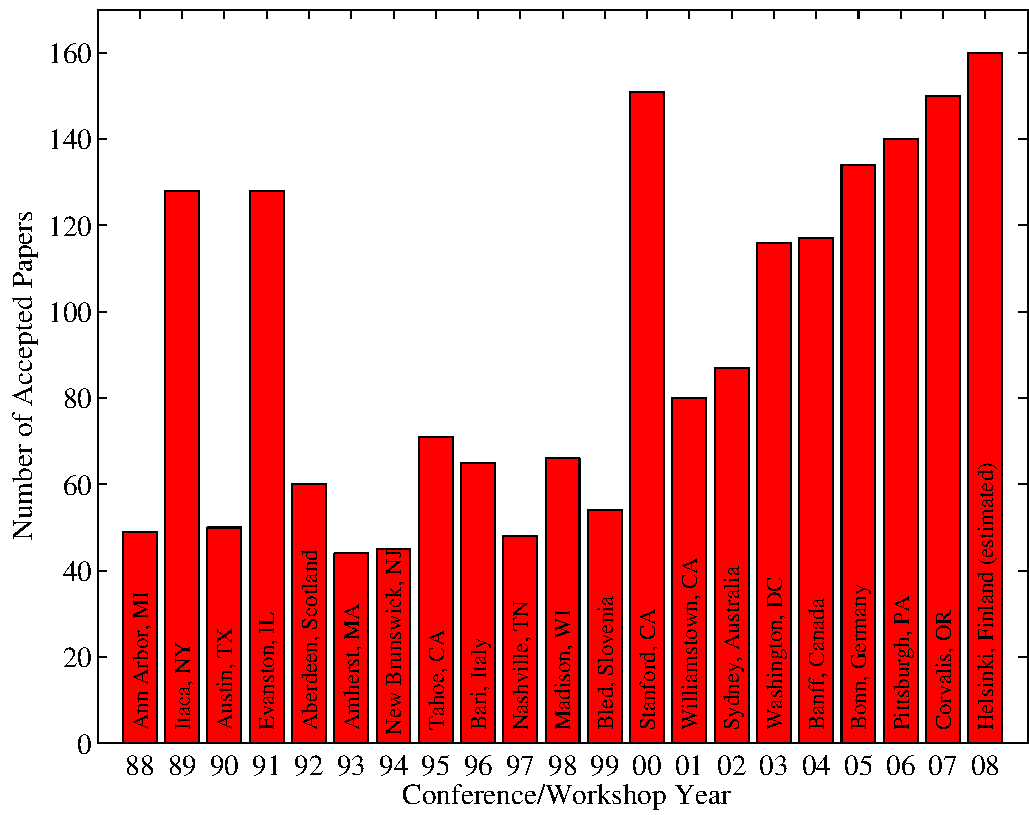
\includegraphics[width=\columnwidth]{icml_numpapers}}
\caption{Historical locations and number of accepted papers for International
Machine Learning Conferences (ICML 1993 -- ICML 2008) and International
Workshops on Machine Learning (ML 1988 -- ML 1992). At the time this figure was
produced, the number of accepted papers for ICML 2008 was unknown and instead
estimated.}
\label{icml-historical}
\end{center}
\vskip -0.2in
\end{figure}
\fi

\bibliography{icml2019}
\bibliographystyle{icml2019}
\end{document}
